\documentclass{article} 
\usepackage{geometry,graphicx,float}
\geometry{
	a4paper,
	total={170mm,257mm},
	left=20mm,
	top=20mm,
}
\linespread{1.5}
\title{Predicting Gene ``Mapk1" in Mice}

\author{
  D'Azevedo, Gloria\\
  \texttt{gad87@cornell.edu}
  \and
  Yadav, Pihu\\
  \texttt{py82@cornell.edu}
}
\date{December 2, 2016}

\begin{document}
\maketitle

%Generate a table of contents for clarity and to use more space if we want.
\tableofcontents

\section{Executive Summary}
The goal of this analysis is to create a model that accurately predicts the value of expressions of gene ``Mapk1".  This is important for aiding cancer diagnosis and treatment in a patient.  An ideal model will depend on a few variables to have low variance when predicting response of the gene on new gene expressions.  The dataset that we are given has 40 gene expressions each with responses from 24 different genes, including ``Mapk1".  A few methods are tried to initially choose the best set of variables such as best subset selection, forward backward subset selection, and regularized regression using lasso.  The Bayesian Information Criterion is minimized to determine the best subset of variables.  Then, the potential sets of models are each fit to ``Mapk1" using non-regularized regression (i.e. least squares) and are evaluated against each other by the Adjusted $R^2$ metric.  The best linear model for predicting ``Mapk1" has 4 variables, $Akt2$, $Rik$, $Pik3r3$, and $Rac1$ and their model has an Adjusted $R^2$ value of 0.5656.  In potential future model development, the problem can be rephrased into a classification problem where instead of predicting the exact expressions of ``Mapk1", the model can predict the range of values for that specific gene so unsupervised methods such as K-Nearest-Neighbors, decision trees, and random forests can be used in addition to linear models.

\section{Introduction and Problem Definition}
The goal of this analysis is to take a gene expression data set for a mouse and develop a model to predict the amount of the gene ``Mapk1".  This gene is very prominent and plays a significant role in cell proliferation.  In general, cells reproduce to make new healthy cells and dispose of older cells; however, an abnormally large amount of cell proliferation can lead to cancerous cells.  If there exists a good (cheap and fast) method to measure the gene creation of proliferating proteins in a patient over time, then the doctors can detect the early onset of cancer and other diseases.  Early diagnosis and the resulting less-invasive treatment usually result in higher survival rate for these patients.  Gene tests in the present day can generally be run to measure the amount of a specific gene in a sample; however, the process can take up to a few days and a sample can only be used once to test the amount of a gene, reliably.  Thus, the goal is to find a model that can accurately predict the amount of the gene  ``Mapk1" with the fewest number of predictors, or other gene tests.\\
\null\\
%
In general, gene analysis is important because they are an indicator for the current and future health issues for the organism as well as the organism's offspring.  However, the procedures to decompose the gene expressions can be expensive and can take a long time, so a model that requires few predictors to predict the value of a certain gene is crucial for accurate and early diagnosis for a potential disease.  In addition, experiments can be done to assess the effects of the presence or absence of specific genes in an organism so cures for these diseases can be developed and doctors know exactly what genes to target to cure their patients.\\
\null\\
%
The data set that is used to develop a model is very small.  There are only 40 different gene expressions, with the responses from 24 genes
in each.  There are no missing values.  The responses are all real numbers, ranging from -2.5 to 2.  Model types to investigate include best subset selection and forward/backward selection for linear model selection (with least squares as the loss function) as well as regularized linear regression.  In addition, resampling methods such as bootstrapping and cross-validation will be extremely useful as there is so little data.  These methods and techniques are generally quite interpretable and the robustness can be tested using the resampling methods mentioned above.\\
\null\\
In addition, for model size selection we use the Bayesian Information Criterion as a measure of model fit that takes into account model size.  The function to calculate the BIC is as follows:
\begin{equation}
BIC=-log(L)+d*log(n)
\label{eq:BIC}
\end{equation}
In Equation \ref{eq:BIC}, $L$ is the value of the likelihood function, $d$ is the number of predictors in the model, and $n$ is the number of data samples.  A smaller value of BIC implies a better model fit.  \\
\null\\
After choosing the correct number and set of predictors and thus identifying the best model for each machine learning technique, we use non-regularized regression (calculated via least squares) to calculate the coefficients for each of the models and evaluate the fits of those using the Adjusted $R^2$ metric. This measures how well the data fits to a linear model but also taking into account the size of the model.  The exact calculation of Adjusted $R^2$ ($R^2_{adj}$)is as follows where $R^2$ denotes the non adjusted $R^2$ and can be found below in Equation \ref{eq:R2}.
\begin{equation}
R^2_{adj} = R^2-(1-R^2)\frac{p}{n-p-1}
\label{eq:AdjR2}
\end{equation}

\begin{equation}
	R^2=1-\frac{\sum_{i=1}^n (y_i-\hat{y_i})^2}{\sum_{i=1}^n (y_i-\bar{y})^2}
	\label{eq:R2}
\end{equation}
%
\section{Model Development}
\subsection{Best Subset Selection Using Linear Models}
There are 23 genes that can be leveraged to predict the response for the ``Mapk1" gene so one of the implemented models is the best subset selection algorithm using exhaustive search.  In this algorithm, all possible $2^r$ linear models are fit to the data using least squares where $r$ is the number of predictors (in this problem, $r=23$).  Then, the algorithm returns the best set of predictors for each model of size 1 to $r$.  Generally, this algorithm is very computationally intensive but since there are only $n=40$ data points so each iteration runs quite quickly on an average computer.  The downside of this algorithm for this data set is that there are only 40 data points, so splitting it further into training and test sets yields poor estimates of the model for each iteration. \\
\null\\
\begin{figure}[H]
	\caption{Best Subset of Predictors for Each Model Size, ordered by increasing BIC}
	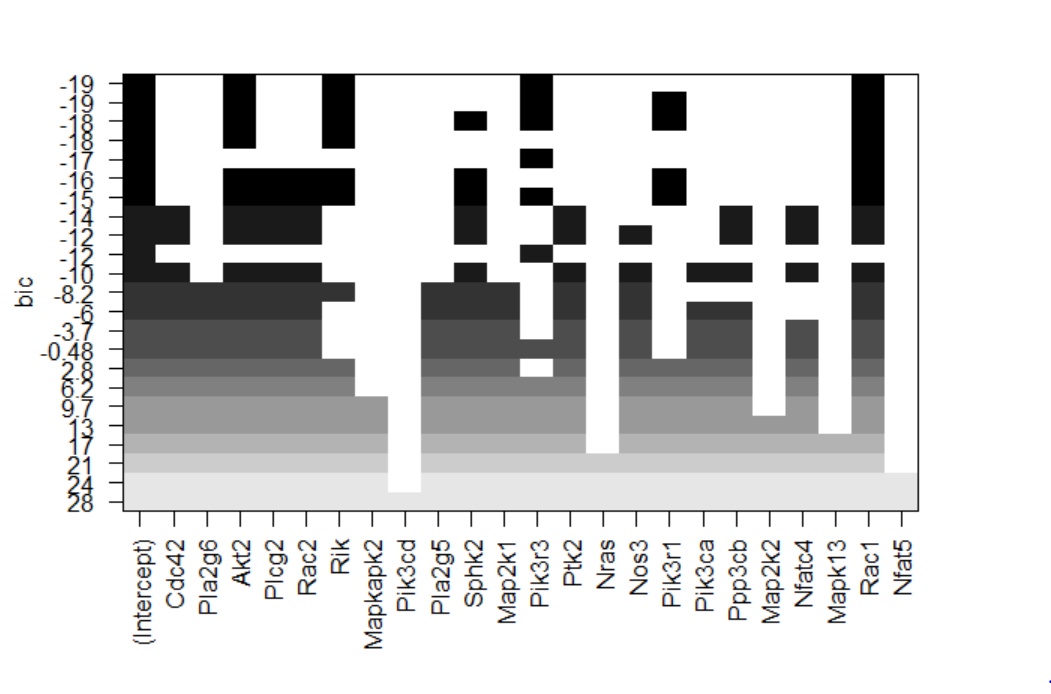
\includegraphics[scale=0.60]{best_subsets}
	\centering
	\label{fig:best_subsets}
\end{figure}
From the chart we determine that the model with the lowest BIC value is the one that includes $Akt2$, $Rik$, $Pik3r3$, and $Rac1$.  The BIC value for the top model (4 predictors) is  -19.2352 while the BIC value for the second best model (5 predictors) is -18.9804 which are both fairly close, if we wanted to consider the 5 predictor model as well.\\
\null\\
While our model is very comprehensive, as it is built using the entire dataset, it is not certain if it is the best model for predicting on new data, data that the model hasn't seen before (test data).
Thus, despite the problems associated with splitting this data further (very few data points), we have implemented a program that performs validation on a test set that the best subset model was not trained on. This program continuously splits the data into training and test data, builds the best subset model prediction for all r maximum allowed parameters on the training data, and fits each of these on the test data to determine the best model. We noticed that on each iteration the model that gave the best test error was generally different, however there was one model that was observed more frequently than the others and was seen to be the best model almost 50\% of the time and this was the model with only 2 predictors: $Pik3r3$ and $Rac1$. This is in contrast to the model built on the entire data which had $Rik$ and $Akt2$ as well.\\
\null\\
From observations made later in the report we see that there is a strong correlation between the genes $Rik$ and $Pik3r3$ as well as $Nfat5$ and $Mapk1$. Hence, since these genes vary together, adding only one of them to the final model should be sufficient and should capture the changes in the outcome gene effectively. This is why our model with only 2 predictors may be considered more effective than other bigger models, of course since it is only being predicted as the best model 50\% of the time, it may not be possible to make a definitive statement on this until we have more data points that can make the testing process more effective. Which is why, presently, it makes sense to only consider the best subset on the entire dataset and get one singular comprehensive model, as given by the model described previously.

%
\subsection{Forward-Backward Model Selection}
The Forward-Backward Model Selection is a variant of the Best Subset Selection which is less computationally expensive.  In the future, if we had more predictors or genes for the model instead of only 23, then this would be a good algorithm to use instead of best subsets as the number of models tested increases linearly instead of exponentially.  The algorithm starts with an initial model and a corresponding objective value (in this case we use the Bayesain Information Criterion (BIC) because it has a larger penalty on larger models).  For each step in the algorithm, models with one more variable than the current model and models with one less variable than the current model are each fit in turn and the BIC is calculated for each.  In other words, if the current size of the model was $k$, then the model fits $23-k$ models of size $k+1$ and $k-1$ models of size $k-1$ and evaluates the objective value of each.  The next step of the algorithm uses the model with the smallest objective value to proceed with the next iteration (which could be the original model of size $k$).  The algorithm finishes when adding or removing a variable from the model would yield a higher BIC value.\\
\null\\
When implementing the forward-backward model selection, we also included Leave-One-Out-Cross-Validation (LOOCV) to have disjoint training and test data.  Obviously if we had more data, then we would use a k-fold cross validation with 5 or 10 folds instead of $n$ folds which is how LOOCV is implemented.  Thus the whole procedure is as follows:\\
\null\\
For each $i=1,\dots, n$:\\
1. Use data point $i$ as the test set and the rest of the data as the training set.\\
2. Perform stepwise forward and backward selection using BIC as the objective value to minimize.\\
3. Calculate the test error using data point $i$. \\
The final optimal model using this method includes $Akt2$, $Rik$, $Rac1$, $Pik3r3$ as the predictors in the linear model.

\subsection{Linear Regression with Regularization}
As an extension to linear regression, we also incorporate a regularizer in order to make the model more robust and determine which predictors are the most significant.  In other words, instead of trying to find the coefficients for the linear model that minimizes the squared errors, we include some bias in the model in order to decrease the variance of the model and prevent overfitting.  This bias of the model is implemented by adding an additional term that is the norm of the predictors to the objective value. This will help ensure that some of the coefficients of the predictors will be exactly $0$, which may not yield the smallest sum of squared differences, but for estimating new data the model will be more accurate. \\
\null\\
For this application, we would like to test and evaluate the fewest number of genes possible as the chemical processes can take a long time.  Thus, we prefer a sparse model so that fewer genes are needed to predict the response gene ``Mapk1" and a model with fewer predictors will have smaller variance.\\
\null\\
The lasso regularizer for linear regression yields sparse models.  When determining the coefficients for this model, we want to minimize the following objective function.  The rows of the input data are denoted by $x_i$ while the whole matrix that is used is $\mathcal{R}^{nxd}$, the output or response for data point $i$ is denoted by $y_i$ and the coefficients for the predictors of the linear model are denoted in the vector $w$ that is made up of components $w_j$ for $j=1,\dots,d$
\begin{equation}
	\textbf{minimize}_w \sum_{i=1}^n(y_i-x_i^Tw)^2+\lambda\sum_{j=1}^d |w_j| = \textbf{minimize}_w \sum_{i=1}^n(y_i-x_i^Tw)^2+\lambda||w||_1
\end{equation}
For this problem with few data points, we use cross validation to find the optimal $\lambda$ value which acts as measure of how much bias the model is able to have.  If $\lambda = 0$ then we get the nonregularized problem, however, if $\lambda$ is too large, then all of the coefficients will go to $0$ to find the minimum objective value.  The $\lambda$ that minimizes the mean cross validated error yields a model with 6 predictors and an intercept and the resulting mean squared error is 0.0121.  We also investigate using the largest $\lambda$ such that error is within 1 standard error of the minimum value of the response.  This yields a smaller model with an intercept and only 4 predictors and a corresponding mean squared error of 0.013. This value is not significantly different from the mean squared error of the $\lambda$ corresponding to the minimum mean squared error of 0.0121 so we still keep it in consideration if we want a simpler model with a slight increase in the mean squared error.  The significant predictors from the simpler model are $Rik$, $Pik3r3$, $Rac1$, and $Nfat5$.  

\section{Results and Conclusions}
Because our outputs are real numbers, we use a squared error loss to evaluate the training error and the test error of our model, but we also want to keep in mind that a simpler model is better even if we have to add some bias to decrease the overall variance of the model.  From the best subset regression, we see that the predictors for the model are $Akt2$, $Rik$, $Pik3r3$, and $Rac1$ (Model 1), when the model is built using the entire dataset. From the forward-backward subset selection with LOOCV, we get a linear model with the same 4 predictors as well: $Akt2$, $Rik$, $Rac1$, $Pik3r3$.  However, when using regularized linear regression, we see that we get a slightly different set of 4 predictors for the model: $Rik$, $Pik3r3$, $Rac1$, and $Nfat5$ (Model 2) when we do not use the $\lambda$ corresponding to the minimum mean squared error but instead use the maximum value of $\lambda$ such that the mean squared error is still within a reasonable bound of the minimum error.  Using this higher value of $\lambda$ gives us a simpler model. \\
\null\\
Investigating this discrepancy between the predictors in each of the models, we note that the gene $Nfat5$ is fairly positively correlated with $Rik$ (the correlation between them is 0.6033). In fact, there is observed to be a strong correlation between all four genes: $Pik3r3$, $Nfat5$, $Map2k1$ and $Rik$. These four also have a strong correlation with the outcome gene and can be considered to be a group of sorts. Thus, if the model includes both the genes $Nfat5$ and $Rik$, then there is not much ``new" information being added. This brings us back to the second model discussed in the Best Subset Regression with a separate training and test set, this model, that was predicted to be the best subset most frequently, had only two predictors: $Pik3r3$ and $Rac1$ (Model 3). Since $Pik3r3$ is strongly correlated with $Nfat5$, $Map2k1$, $Rik$ and the outcome gene (and they are all correlated with each other), it may be sufficient to include only $Pik3r3$ to take into account the effect of that all of them have on the outcome gene ($Mapk1$).  \\
\null\\
Fitting a non regularized linear model to each of the aforementioned Models 1,2 and 3, we get the following equations:
\begin{equation}
	Mapk1 = -0.44461-0.40548Akt2+0.22072Rik+0.24399Pik3r3+0.31716Rac1
	\label{eq:Model1}
\end{equation}
All the predictors in Model 1 are significant to the model, and $R^2_{adj}=0.5656$.\\
\null\\
For Model 2 we get the following equation:
\begin{equation}
	Mapk1=-0.3109+0.1741Rik+0.2331Pik3r3+0.2570Rac1+0.0864Nfat5
	\label{eq:Model2}
\end{equation}
In Model 2, only $Rac1$ is significant to the model at the 0.001 significance level and $Pik3r3$ is significant at the 0.1 significance level and $R^2_{adj}=0.4998$.
For Model 3 we get the following equation:
\begin{equation}
	Mapk1=-0.05643+0.40410Pik3r3+0.27832Rac1
	\label{eq:Model3}
\end{equation}
In Model 3, both the predictors are highly significant, with Pik3r3 at the 0 significance level and Rac 1 as the 0.001 significance level. $R^2_{adj}=0.4777$, which is lower than what we are getting for Model 1 and Model 2. \\
\null\\
The non-significance of most of the predictors in Model 2 may be partially caused by the high correlation between $Nfat5$ and the other predictors. The value of adjusted R squared for this model is lower than Model 1.\\
\null\\
In Model 3, while we are getting both the predictors to be highly significant, the value of adjusted R squared is lower than the other models. This may be because the model is too simplistic, and is thus underfitting the data. It is possible that Model 3 might actually be better, but since the Best Subset Regression model with test sets only predicted this to be the best model less than half the times, it would be difficult to make any concrete conclusions in the absence of more data, that would allow test set validation to be performed better. Thus, we conclude that Model 1 is the best at fitting the data to the linear model to predict $Mapk1$.\\
\null\\
Hence, our final recommendation as justified above is to use Model 1 which is comprised of the gene predictors $Akt2$, $Rik$, $Pik3r3$, and $Rac1$.
\begin{equation}
	Mapk1 = -0.44461-0.40548Akt2+0.22072Rik+0.24399Pik3r3+0.31716Rac1
	\label{eq:Model1}
\end{equation}
We also note the degrees of freedom of these models are low since there are only 40 data points and the model needs to estimate 5 coefficients (intercept and 4 variables).  Since there are so few degrees of freedom, we may instead want to assume that the errors are from a student-t distribution instead of a normal distribution to get a more conservative estimate.
%
\begin{table}[!htbp] \centering 
	\caption{Summary table of models and their coefficients} 
	\label{table:results} 
	\begin{tabular}{@{\extracolsep{5pt}}lcccc} 
		\\[-1.8ex]\hline 
		\hline \\[-1.8ex] 
		Model Name & Model Varibles & Adjusted $R^2$ & Residual Standard Error\\ 
		\hline \\[-1.8ex] 
		Model 1 & Akt2, Rik, Pik3r3, Rac1 & 0.5656 & 0.08281 \\ 
		Model 2 & Rik*, Pik3r3*, Rac1, Nfat5* & 0.4998 & 0.08886 \\ 
		Model 3 & Pik3r3, Rac1 & 0.4777 & 0.0908\\ 
		\hline \\[-1.8ex] 
		* Denotes non-significant predictors in model 
	\end{tabular} 
\end{table} 

\section{Next Steps}
In the future, if data is collected for more mice and there are more gene expressions to analyze, we may be able to use test data as a better indicator of the accuracy of our models. With the present data, we got variable results from training and testing on separate sets, which may be due to the fewer number of data points available. In this case, other methods such as K-Nearest-Neighbors (KNN) or fitting polynomial splines can be implemented. KNN is a robust, unsupervised machine learning technique.  Currently, as there are only $40$ samples, the number of points that have k nearest neighbors is at most $40-k$, assuming that the whole data set is used as a training set and none of it is used to evaluate the model and estimate test error.  If KNN is implemented on the current data, the model overfits to the training data, consequently yielding a low training error, which does not imply a low test error for new samples.  Fitting piecewise polynomials to the data may also be useful if the data is inherently nonlinear, which we have assumed so far.  \\
\null\\
In addition, in the real health diagnosis setting, there may be predefined ranges of the amounts of the gene/protein that is classified as a normal range, a warning range, and a dangerous range.  In that case, we can reframe the problem as ordinal classification and use methods such as KNN, decision trees, or other machine learning techniques.  These methods are more variable in terms of model training and some sort of resampling method will still have to be used since there is not much data present. 
\end{document}
